%%%%%%%%%%%%%%%%%%%%%%%%%%%%%%%%%%%%%%%%%
% University/School Laboratory Report
% LaTeX Template
% Version 3.0 (4/2/13)
%
% This template has been downloaded from:
% http://www.LaTeXTemplates.com
%
% Original author:
% Linux and Unix Users Group at Virginia Tech Wiki 
% (https://vtluug.org/wiki/Example_LaTeX_chem_lab_report)
%
% License:
% CC BY-NC-SA 3.0 (http://creativecommons.org/licenses/by-nc-sa/3.0/)
%
%%%%%%%%%%%%%%%%%%%%%%%%%%%%%%%%%%%%%%%%%

%----------------------------------------------------------------------------------------
%	PACKAGES AND DOCUMENT CONFIGURATIONS
%----------------------------------------------------------------------------------------

\documentclass{article}

\usepackage{mhchem} % Package for chemical equation typesetting
\usepackage{siunitx} % Provides the \SI{}{} command for typesetting SI units
\usepackage{listings}
\usepackage{commath}
\usepackage{verbatim}
\usepackage{graphicx} % Required for the inclusion of images
\usepackage[margin=1in]{geometry}
\usepackage{multirow}
\usepackage{array}
\setlength\parindent{0pt} % Removes all indentation from paragraphs


%\usepackage{times} % Uncomment to use the Times New Roman font

%----------------------------------------------------------------------------------------
%	DOCUMENT INFORMATION
%----------------------------------------------------------------------------------------

\title{ Homework 2 \\ COSC 594} % Title

\author{Jiahui \textsc{Guo}} % Author name

\date{\today} % Date for the report

\begin{document}

\maketitle % Insert the title, author and date

% If you wish to include an abstract, uncomment the lines below
% \begin{abstract}
% Abstract text
% \end{abstract}

%----------------------------------------------------------------------------------------
%	SECTION 1
%----------------------------------------------------------------------------------------

\section{Program Implementation}

\subsection{Test Data}
The matrices are initialized with random number ranging from 0 to 100 with double type. 

\subsection{Program Organization}
The program is organized in the following way:
\begin{description}
    \item[src]/
        \begin{description}
            \item[omp\_gemm.c]
            \item[omp\_trsm.c]
            \item[c\_timer.c]
            \item[Makefile] 
        \end{description}
    \item[include]/
        \begin{description}
            \item[c\_timer.h]
        \end{description}
    \item[bin]/
        \begin{description}
            \item[run.sh] Run the executable files and generates plots
            \item[avg.py] 
            \item[plotTime.gnu]
        \end{description}
    \item[Makefile]
    \item[ReadMe] Illustrating how to execute the program.
\end{description}

\newpage
\section{Experiment Platform}
The experiment was conducted on a hydra machine. The configuration of the machine is list below:
\begin{description}
\item[Processor] Intel Core i7-3770 $@$ 3.40GHz
\item[Memory] 16.0GB DDR3
\item[Hard drive] 500GB 7200 RPM SATA $@$ 6Gbps, 16MB cache
\item[Thread(s) per Core] 4
\item[Core(s) per socket] 2
\item[Socket(s)] 1
\end{description}

\newpage
\section{Approaches}
\subsection{GEMM}
This program implements the GEMM, which is defined as:
\begin{equation*}
C \leftarrow \alpha AB + \beta C
\end{equation*}

Then the program is executed with different parameter settings,  which are listed below:
\begin{itemize}
\item Matrix Size: From 100 to 3000 with step size 100
\item Chunk Size: 10 and 50
\item Number of Threads: 4 and 8
\item Schedule Type: Static and dynamic
\end{itemize}

\subsection{TRSM}
The TRSM short for TRiangular Solve with Matrix,  it solve the following problem:
\begin{equation*}
AX = B
\end{equation*}
where $A$ is either upper or lower triangular, and the solution matrix $X$ is returned in the space
occupied by $B$.

\newpage
\section{Obtain OpenMP environment information}
Information of OpenMP environment is obtained through the following built-in function:
\begin{table}[h]
\begin{center}
\begin{tabular}{| l | l |}
\hline
Number of processors available & \verb+omp_get_num_procs()+\\
\hline
Number of threads being used & \verb+omp_get_num_threads()+\\
\hline
Set the number of threads & \verb+omp_set_num_threads(NTHREADS)+\\
\hline
Maximum number of threads available & \verb+omp_get_max_threads()+\\
\hline
If in parallel region & \verb+omp_in_parallel()+ \\
\hline
If dynamic threads are enabled & \verb+omp_get_dynamic()+\\
\hline
If nested parallelism is supported & \verb+omp_get_nested()+\\
\hline
\end{tabular}
\end{center}
\end{table}

All the information would be printed to shell if the DEBUG macro is uncommented in source code.

\newpage
\section{Experiment Results}
\subsection{GEMM}
The experiments results using diffrent parameter settings for gemm are shown in Fig.1 to Fig.9.

    \begin{figure}[th!]
        \centering
        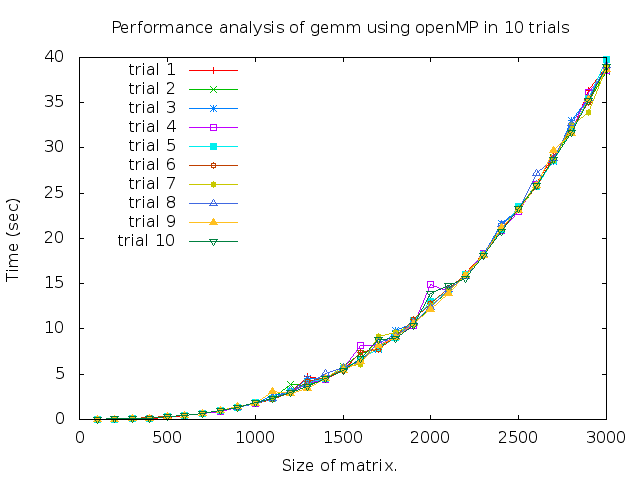
\includegraphics[width=0.8\textwidth]{static_ck10_8.png}
        \label{fig:1}
        \caption{Execution time with static schedule, 8 threads, chunk size 10 in 10 trials}
    \end{figure}

    \begin{figure}[th!]
        \centering
        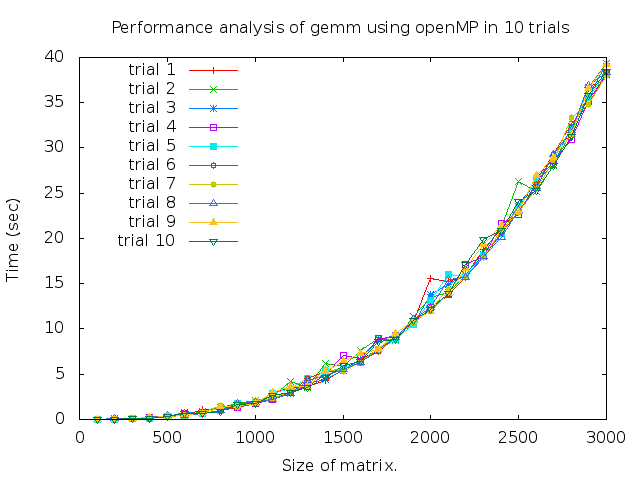
\includegraphics[width=0.8\textwidth]{static_ck10_4.png}
        \label{fig:2}
        \caption{Execution time with static schedule, 4 threads, chunk size 10 in 10 trials}
    \end{figure}
    
    \begin{figure}[th!]
        \centering
        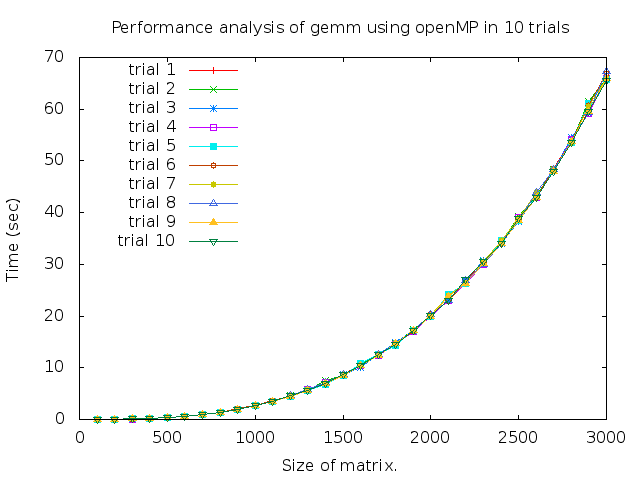
\includegraphics[width=0.8\textwidth]{static_ck10_2.png}
        \label{fig:3}
        \caption{Execution time with static schedule, 2 threads, chunk size 10 in 10 trials}
    \end{figure}
    \begin{figure}[th!]
        \centering
        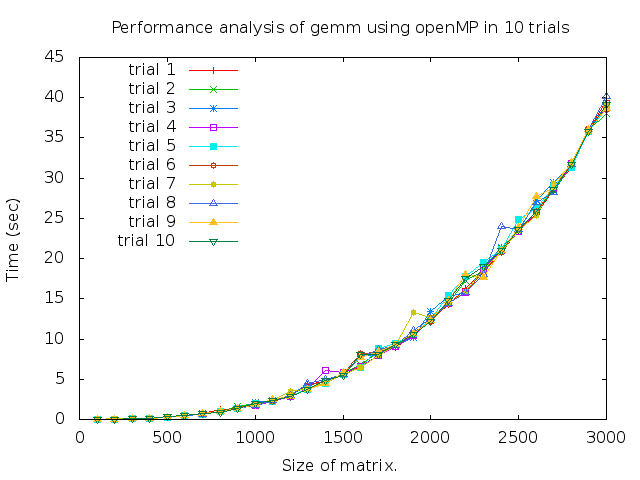
\includegraphics[width=0.8\textwidth]{static_ck50_8.png}
        \label{fig:4}
        \caption{Execution time with static schedule, 8 threads, chunk size 50 in 10 trials}
    \end{figure}

    \begin{figure}[th!]
        \centering
        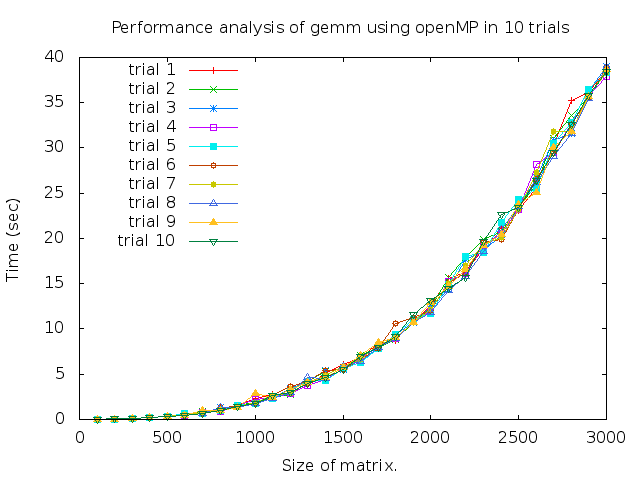
\includegraphics[width=0.8\textwidth]{static_ck50_4.png}
        \label{fig:5}
        \caption{Execution time with static schedule, 4 threads, chunk size 50 in 10 trials}
    \end{figure}

    \begin{figure}[th!]
        \centering
        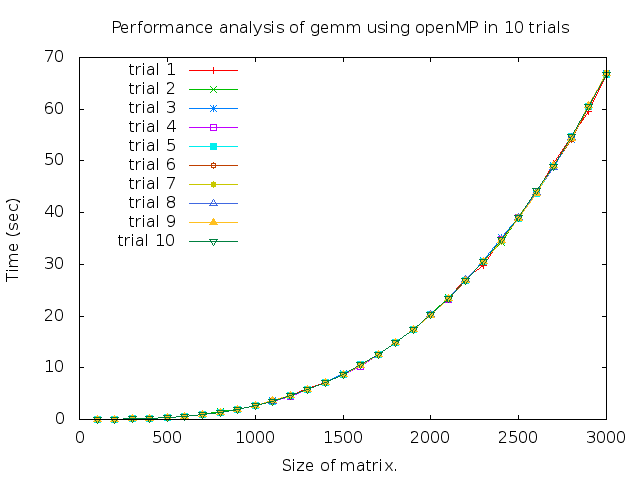
\includegraphics[width=0.8\textwidth]{static_ck50_2.png}
        \label{fig:6}
        \caption{Execution time with static schedule, 2 threads, chunk size 50 in 10 trials}
    \end{figure}

    \begin{figure}[th!]
        \centering
        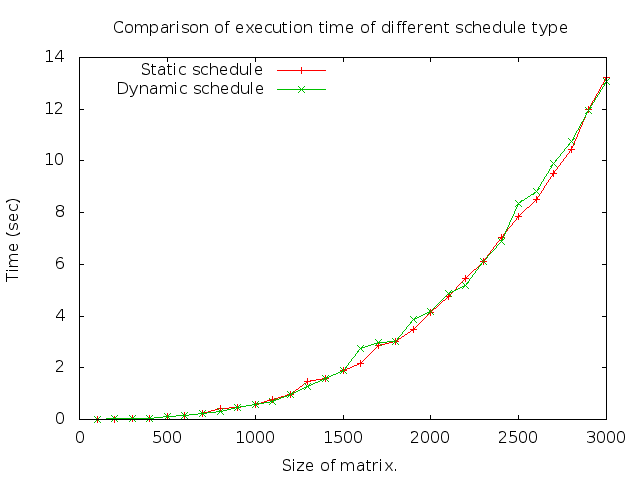
\includegraphics[width=0.8\textwidth]{ck50_8.png}
        \label{fig:7}
        \caption{Comparison of execution time with diffrent schedule, 8 threads, chunk size 50}
    \end{figure}
    
    \begin{figure}[th!]
        \centering
        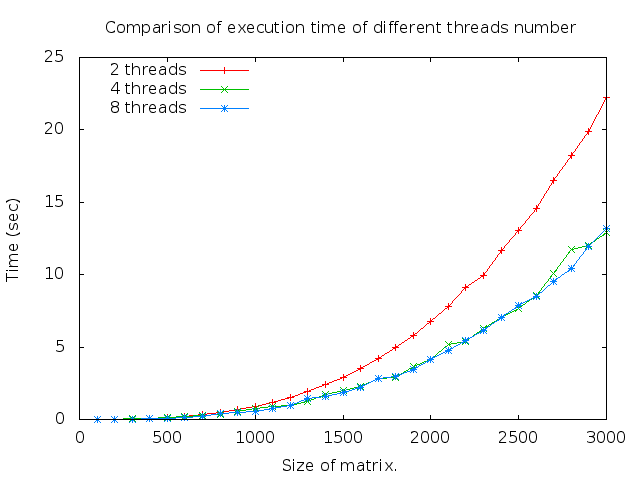
\includegraphics[width=0.8\textwidth]{static_ck50.png}
        \label{fig:8}
        \caption{Comparison of execution time with static schedule, different threads, chunk size 50}
    \end{figure}

    \begin{figure}[th!]
        \centering
        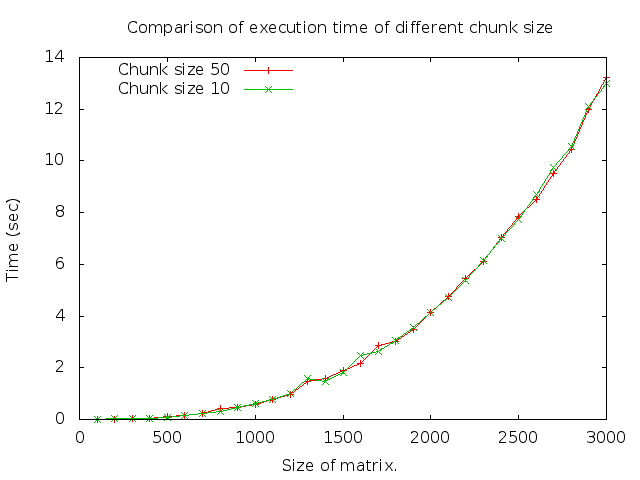
\includegraphics[width=0.8\textwidth]{static_8.png}
        \label{fig:9}
        \caption{Comparison of execution time with static schedule, 8 threads, different chunk size}
    \end{figure}

\newpage
\subsection{TRSM}
The experiments results using diffrent parameter settings for trsm are shown in Fig.10 to Fig.11.

    \begin{figure}[th!]
        \centering
        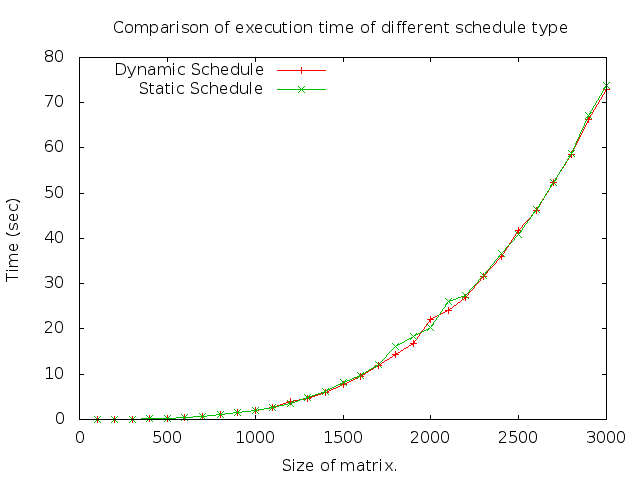
\includegraphics[width=0.8\textwidth]{ck10_8_trsm.png}
        \label{fig:10}
        \caption{Comparison of execution time with diffrent schedule, 8 threads, chunk size 10}
    \end{figure}

    \begin{figure}[th!]
        \centering
        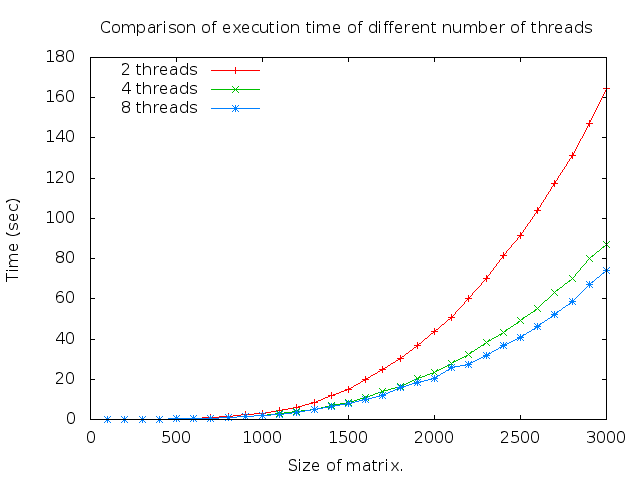
\includegraphics[width=0.8\textwidth]{static_ck10_trsm.png}
        \label{fig:11}
        \caption{Comparison of execution time with static schedule, differentf number of threads, chunk size 10}
    \end{figure}

\newpage
\newpage
\section{Performance discussions}

    \begin{figure}[th!]
        \centering
        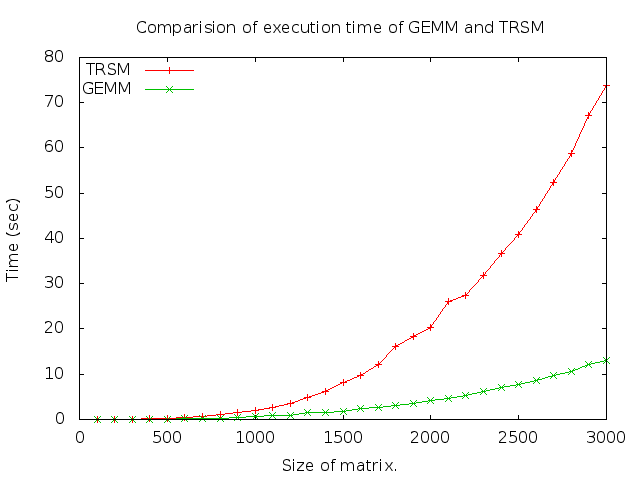
\includegraphics[width=0.8\textwidth]{static_ck10_8_trsm.png}
        \label{fig:12}
        \caption{Comparison of execution time of gemm and trsm}
    \end{figure}

\subsection{Schedule Type}
From the results shown Fig.7 and Fig.10, it seems that the schedule type does not have influence on the execution 
time for GEMM or TRSM. 
\subsection{Chuck Size}
From the results shown Fig.9, it seems that that the chunk size does not have influence on the execution 
time for GEMM. 
\subsection{Threads Number}
Threads number has huge impacts on the execution time of a certain program. In GEMM, from Fig.8 we can see that the
execution time for 4 and 8 threads are almost the same, but for 2 threads, the execution time nearly doubled when the 
matrix size increased to 3000. And in TRSM, from Fig.11, we can also the similar phenomenon.
\subsection{Problem related}
Fig.12 shows the execution time for GEMM and TRSM, using 8 threads, static schedule and chunk size 10, the result
shows that with the increase of the input data size, the runtime for TRSM increases rapidly comparing to GEMM, the 
reason is in GEMM, all the multiplication can be parallel perfectly, but in TRSM, there are dependency for some elements
in the matrix, thus TRSM cannot reach the same throughout as GEMM.

\end{document}
